\documentclass[serif,mathserif,final]{beamer}
\mode<presentation>{\usetheme{Lankton}} 
\usepackage{amsmath,amsfonts,amssymb,pxfonts,eulervm,xspace}
\usepackage{graphicx, ragged2e}
\graphicspath{{./figures/}}
\usepackage[orientation=landscape,size=a0,scale=1.6,debug]{beamerposter}

%-- Header and footer information ----------------------------------
\newcommand{\footleft}{Supercomputing 2012}
\newcommand{\footright}{\today}
\title{Slack-conscious Lightweight Loop Scheduling for Improving Scalability of Bulk-synchronous MPI Applications}
\author{Vivek Kale$^1$$^2$ \quad Todd Gamblin$^2$ \quad Torsten Hoefler$^1$
\quad Bronis R. de Supinski$^2$ \quad William D. Gropp$^1$}
\institute{$^1$ University of Illinois at Urbana-Champaign 
\quad $^2$Lawrence Livermore National Laboratory} 

%------------------------------------------------------------------
%-- Main Document ------------------------------------------------- 
\begin{document}
\begin{frame}{}
  \begin{columns}[t]
    %-- Column 1 ---------------------------------------------------
    \begin{column}{0.33\linewidth} 
      %-- Block 1-1 
      \begin{block}{\small Noise Amplification Problem }
        \begin{figure}[htb] 
          \centering 
          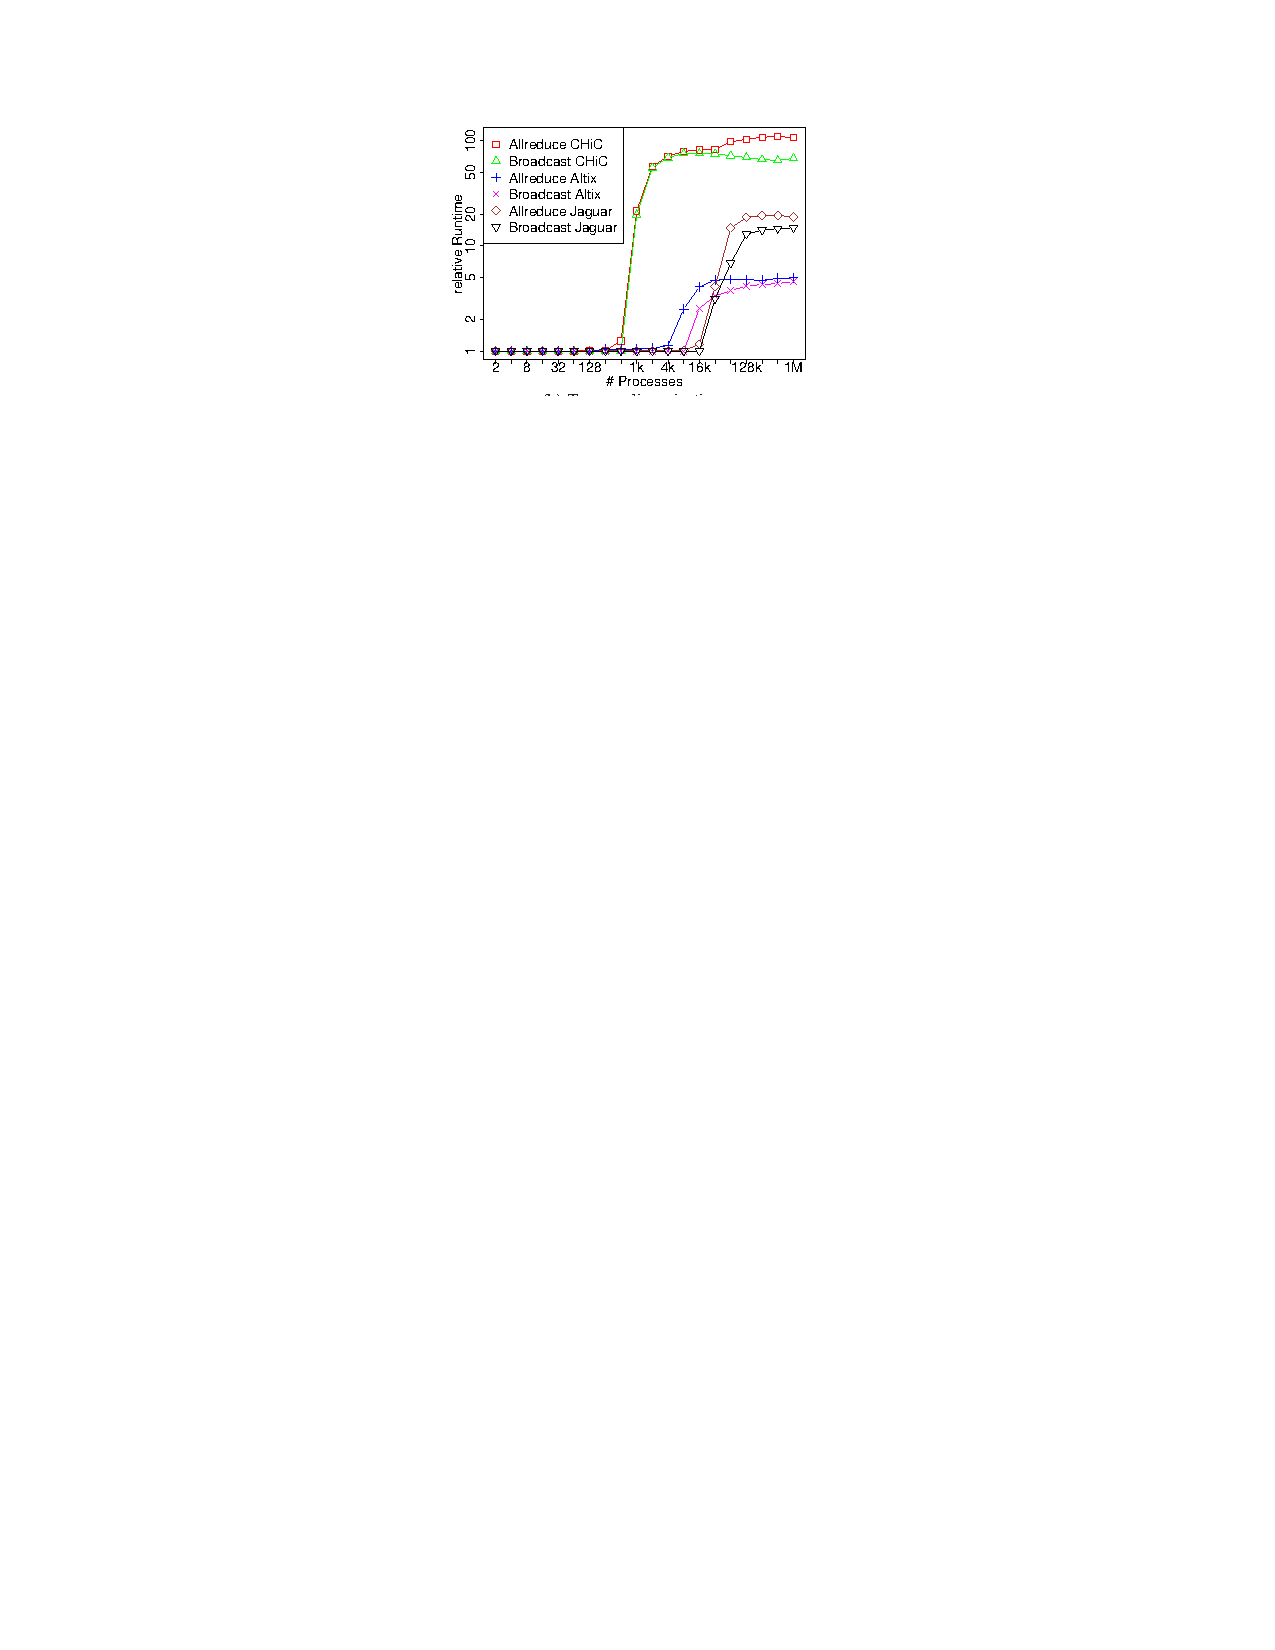
\includegraphics[width=.83\columnwidth]{images/NoiseAmpProblem-sim} 
          \caption{\tiny Effects of Noise Amplification seen at simulation of over 1 million MPI processes.} 
        \end{figure} 
      \end{block} 

      %-- Block 1-2
      \begin{block}{\small Noise Amplification Problem} 
       \begin{columns}[t]
         \begin{column}{0.5\columnwidth}
           \begin{figure}[htb]
             \centering
             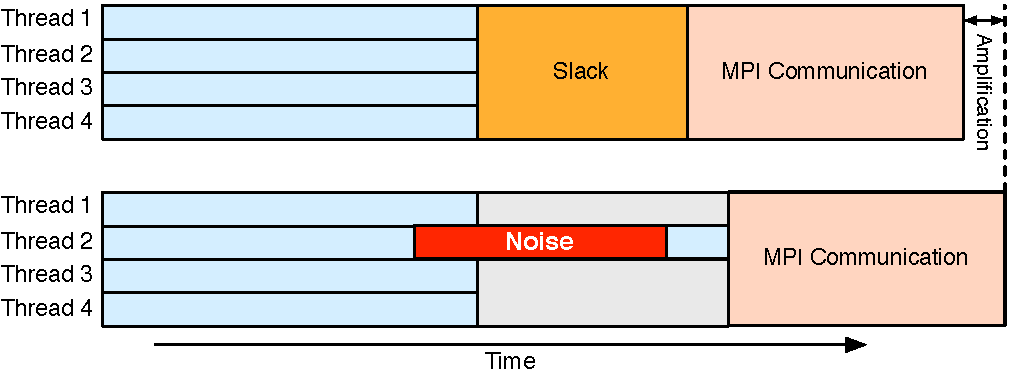
\includegraphics[width=0.9\columnwidth]{images/static-schedule}
             \caption{ \tiny  In one particular application timestep, the 
               local within-node noise can be ``heard'' 
               by another node. } 
           \end{figure}
         \end{column}   
 
         \begin{column}{0.5\columnwidth}
           \begin{figure}[htb] 
             \centering 
             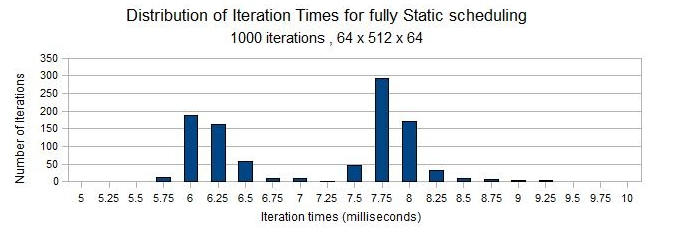
\includegraphics[width=0.9\columnwidth]{images/IterTimingsHisto-static}
             \caption 
                 {
                   \tiny Spread of iteration timings over 1000 iterations of a stencil computation. The first peak represents unperturbed iterations, 
                   and the second peak represents perturbed iterations by noise event. The noise event is not guaranteed to be occur at the same 
                   time across all nodes(e.g. no co-scheduling). 
                 } 
           \end{figure} 
         \end{column}
       \end{columns}
      \end{block} 

%-- Block 1-3 
      \begin{block}{\small Using Lightweight Scheduling to scale past the Noise Amplification Problem}  
       \begin{columns}[t]
         \begin{column}{0.5\columnwidth}
           \begin{figure}[htb]
             \centering
             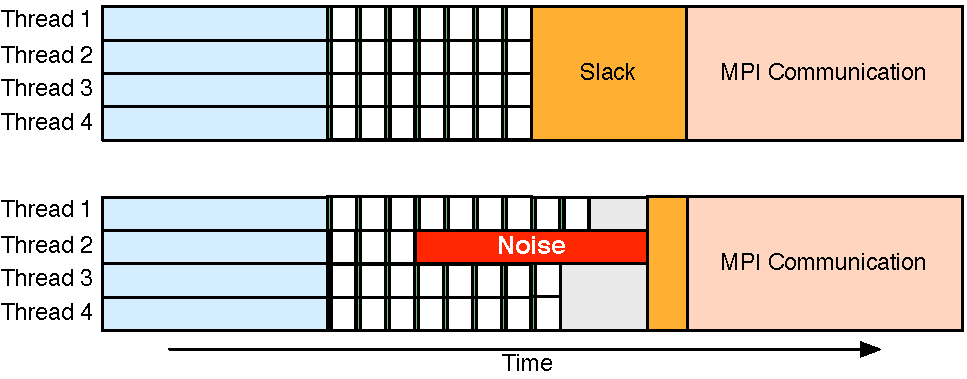
\includegraphics[width=0.9\columnwidth]{images/dynamic-schedule}
           \caption{ \tiny  In one particular application timestep, the 
              local within-node noise can be ``heard'' 
               by another node. } 
           \end{figure}
         \end{column} 
      \begin{column}{0.5\columnwidth}
        \begin{figure}[htb] 
          \centering 
          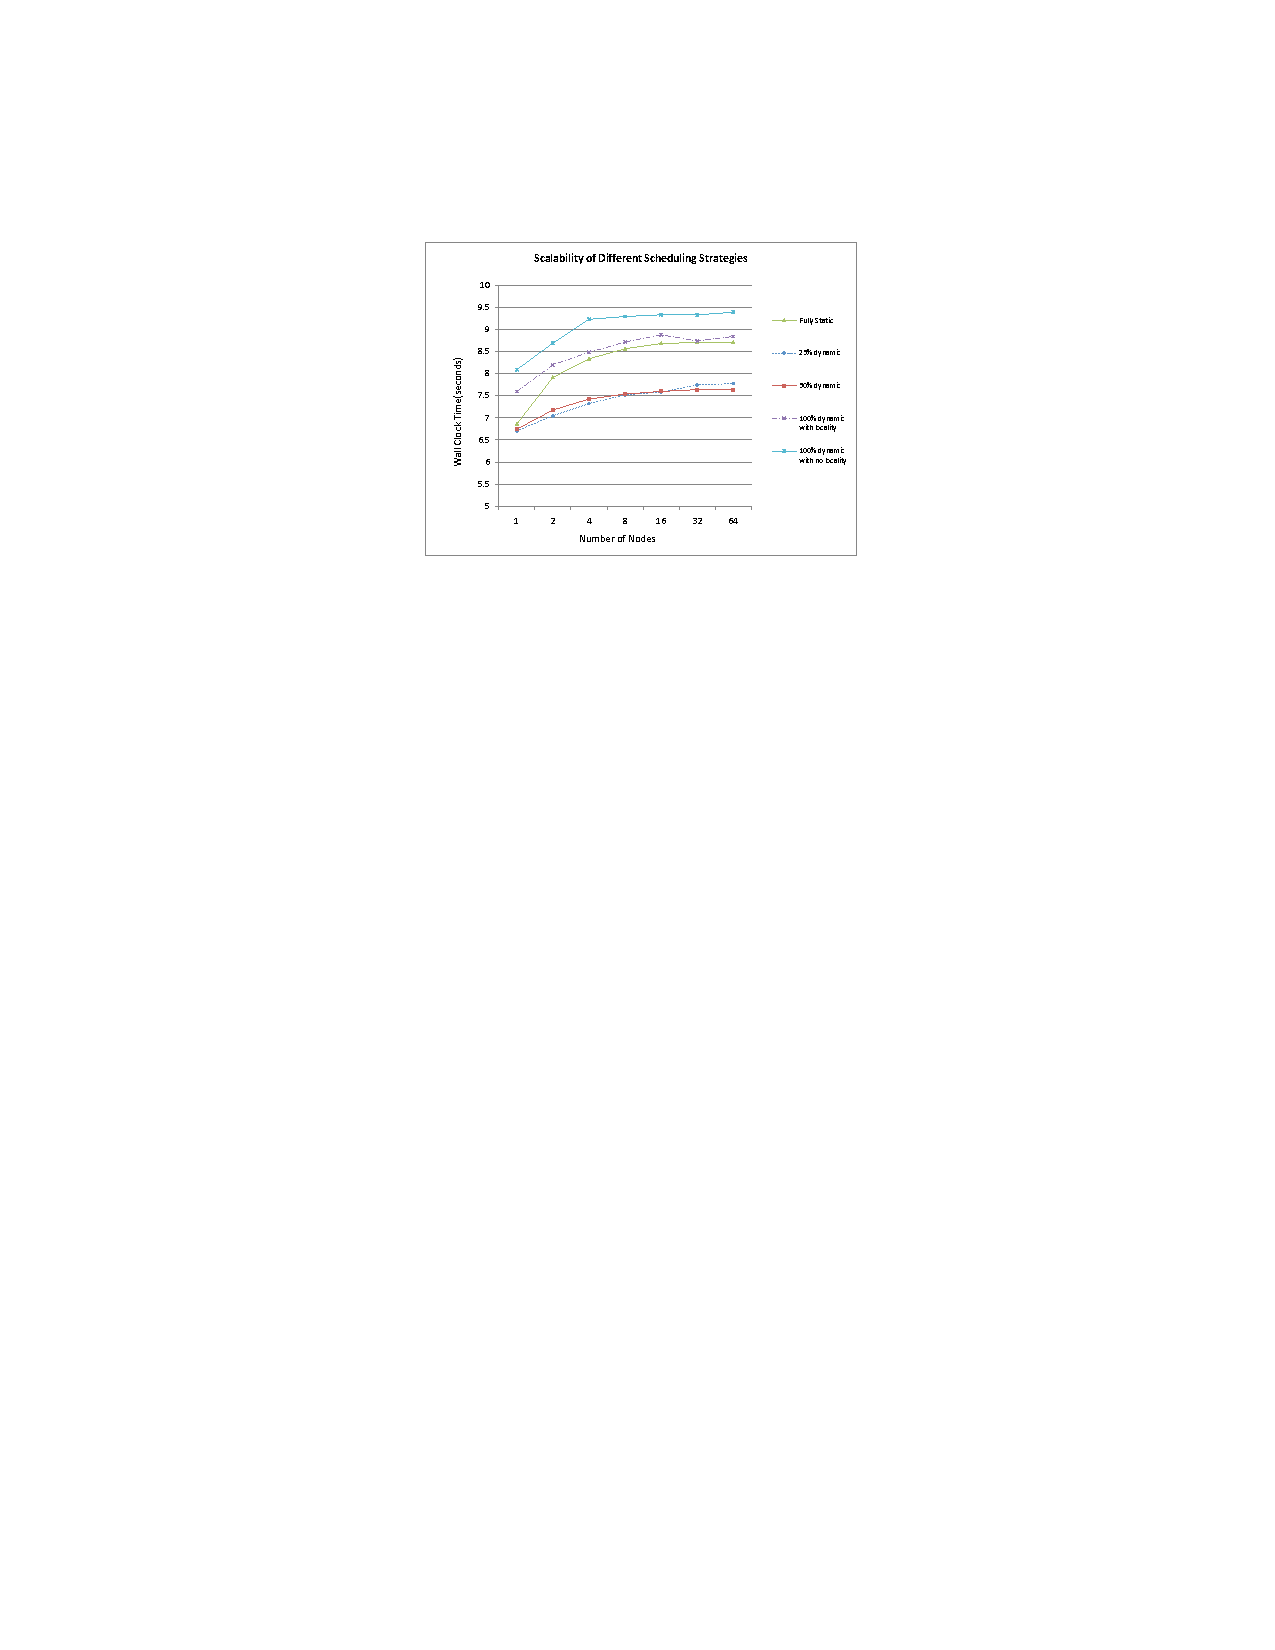
\includegraphics[width=.9\columnwidth]{images/uSched-scaling}
          \caption{  } 
        \end{figure} 
      \end{column} 

         \end{columns}
\end{block}

      
%      \begin{column}
%         \begin{equation*}
%           f_s = 1 - \frac{\delta}{T_p}
%         \end{equation}
%      \end{column}
      
%       \end{columns}
       
%      \end{block} 
      \end{column} %1 

%-- Column 2 ---------------------------------------------------  
\begin{column}{0.27\linewidth} 

%-- Block 2-1 

\begin{block}{\small \textit{Slack-Conscious} Lightweight Work Stealing for Mitigation of Noise Amplification} 
%        \begin{enumerate}
%        \item Certain nodes amplify their noise more than others. 
%        \item The reason is that there is existence of process slack ,i.e., variation in time spent blocking, across all MPI processes. 
%        \end{enumerate} 
%        \textit{Research Question: Can we further increase the static fraction on those nodes not on the critical path of computation?} 

\begin{table}
%\caption{\label{terminology}Definitions of variables used in Theoretical Analysi}
\begin{tabular} {|c|p{24cm}|} \hline
\textbf{\tiny Variable} & \textbf{\tiny Definition} \\ \hline
\tiny $t_{ovhd}$ &  \tiny total overhead of scheduler. \\ \hline
\tiny $t_{ovhdPlus}$ &  \tiny Additional unexpected overhead of scheduler (e.g. due to off-chip coherence cache miss). \\ \hline 
\tiny $t_{noise}$ & \tiny length of time spent per application timestep in noise, by one node.  \\ \hline
%\tiny $n$ & \tiny \# of nodes. \\  \hline
\tiny $p$ & \tiny  \# of cores per node. \\ \hline
%$q$ & \small MPI process number identifier. \\ \hline
%\tiny $pred\_slack\_q$ & \tiny  Predicted slack on rank $q$ (through runtime tool such as Adagio). \\ \hline 
%$max\_slack\_q$ & \small Maximum slack possible across all MPI processes (determined through slack distribution).\\  \hline
\tiny ${\tau}$ & \tiny Tasklet size in terms of number of FLOPs. \\ \hline  
\tiny ${d}$ & \tiny Expected number of tasklets per core. \\ \hline 
\tiny ${\delta}_q$ & \tiny Maximum length of noise across all noise events on rank q. \\  \hline 
% \tiny $T_{p_{q}}$ & \tiny The amount of time for computation and scheduling overhead needed 
% for rank $q$, for one application timestep.  \\ \hline 
% \tiny $T_n$ &  \tiny The amount of total execution time for one application timestep, across all $n$ MPI processes. \\ \hline 
\tiny $\bar{\mathbb{s}}$ &  \tiny The original static fraction with no consideration of MPI slack. \\  \hline 
\tiny $\bar{s}$ (also ${f_s}_{max}$) & \tiny The original ``global'' static fraction with no consideration of MPI slack. \\ \hline 
\tiny $\hat{s_q}$ (also ${f_s}_{q}$) & \tiny The static fraction with consideration of the MPI slack value. This
static fraction is different for each node (depending on slack) and so is identified by subscript $q$. \\ \hline
\end{tabular}
\end{table} 

\end{block}

% -- Block 2-2 
% \begin{block}{Slack-Conscious Lightweight Work-stealing (Performance Model for System Noise and Scheduling Overhead)} 

\begin{block}{}
  \begin{equation*}  
   \tiny t_{ovhd}(f_s) = d \times  ({t_q +  t_{cacheMiss}}
  \end{equation*} 
\end{block} 

\begin{block}{}
  \begin{equation*}
   \tiny t_{noise}(f_s) = \left(\left(2 - \frac{f_s}{{f_s}_{max}}\right) \times \frac{\delta}{p-1} \right)  + \left( \left(\frac{f_s}{{f_s}_{max} - 1}\right) \times \delta \right)  
  \end{equation*} 
\end{block} 

%  $$t_{parallelizedNoise}(f_s) = \left(1.0 - \frac{f_s}{{f_s}_{max}} - 1.0\right) \times \frac{\delta}{p-1}$$  \\
%  $$t_{serializedNoise}(f_s) = \left(\frac{f_s}{{f_s}_{max}} - 1.0\right) \times \delta$$  \\  
%% $t_{noise}$ = \left(\left(2- \frac{f_s}{{f_s}_{max}}\right) \times \frac{\delta}{p-1} \right)  + \left( \left(\frac{f_s}{{f_s}_{max} - 1}\right) \times \delta \right ) 
%\end{block} 
%\begin{block}{Theoretical Analysis of Static Fraction} 

\begin{block}{}
  \begin{equation*}
    \tiny  f_s = \max{ f_s} 
  \end{equation*}
  such that 
  \begin{equation*}
    \tiny t_{ovhd}(f_s) + t_{noise}(f_s) < pred\_slack 
  \end{equation*} 
\end{block} 

%-- Block 2-3 
\begin{block}{\small Slack-Conscious Lightweight Scheduling Runtime System Operation} 
  \begin{figure}[htb]
    \centering
    \includegraphics[width=.67\columnwidth]{images/hybrid-schedule}
    \caption{
\small   The local within-node noise is absorbed through work-stealing. The work-stealing 
      itself can create amplification, so it is done in a low-overhead manner. 
    }
  \end{figure} 
\end{block} 

\end{column}%2 

   %-- Column 3 ------------------------------------------------ 

\begin{column}{0.27\linewidth} 
  %-- Block 3-1 
  \begin{block}{\small Performance Improvement on atlas} 
    \begin{figure}[htb] 
      \centering 
      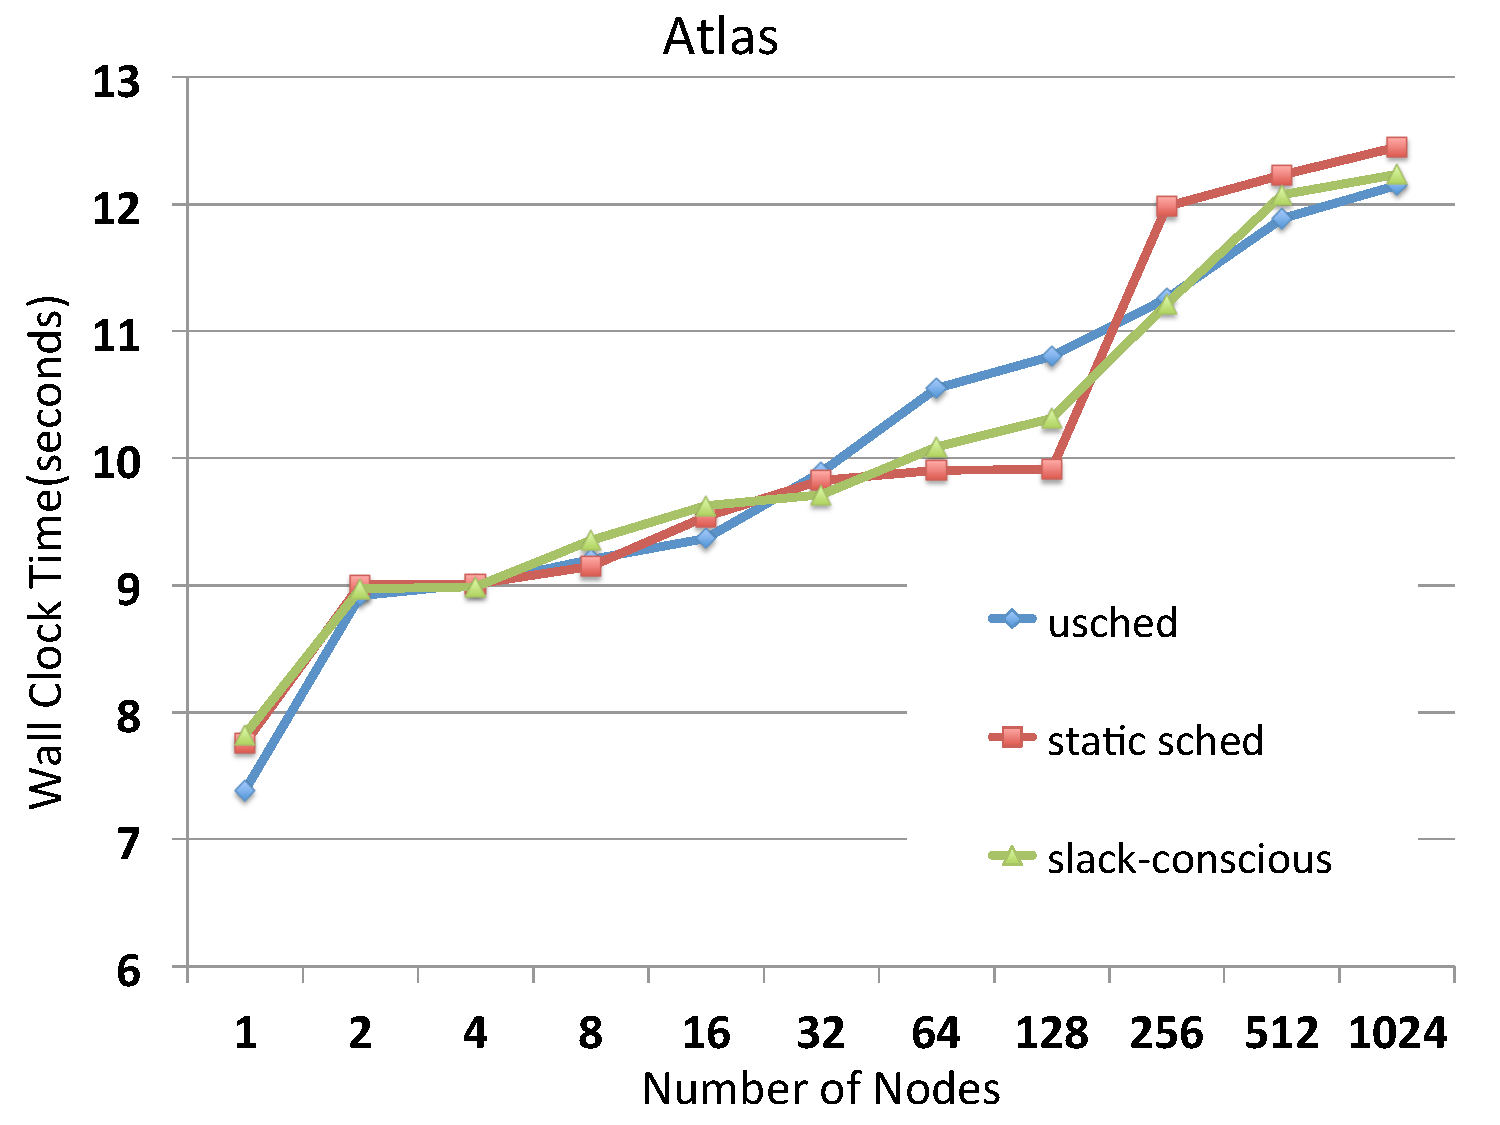
\includegraphics[width=.65\columnwidth]{images/AMG-scaling-atlas}
      \caption{\small On a machine with 8 cores and high noise, slack-conscious lightweight scheduling allows for roughly 3\% perf gains over baseline.} 
    \end{figure} 
  \end{block} 

  %--- Block 3-2
  \begin{block}{\small Performance Improvement on hera} 
    \begin{figure}[htb] 
      \centering
      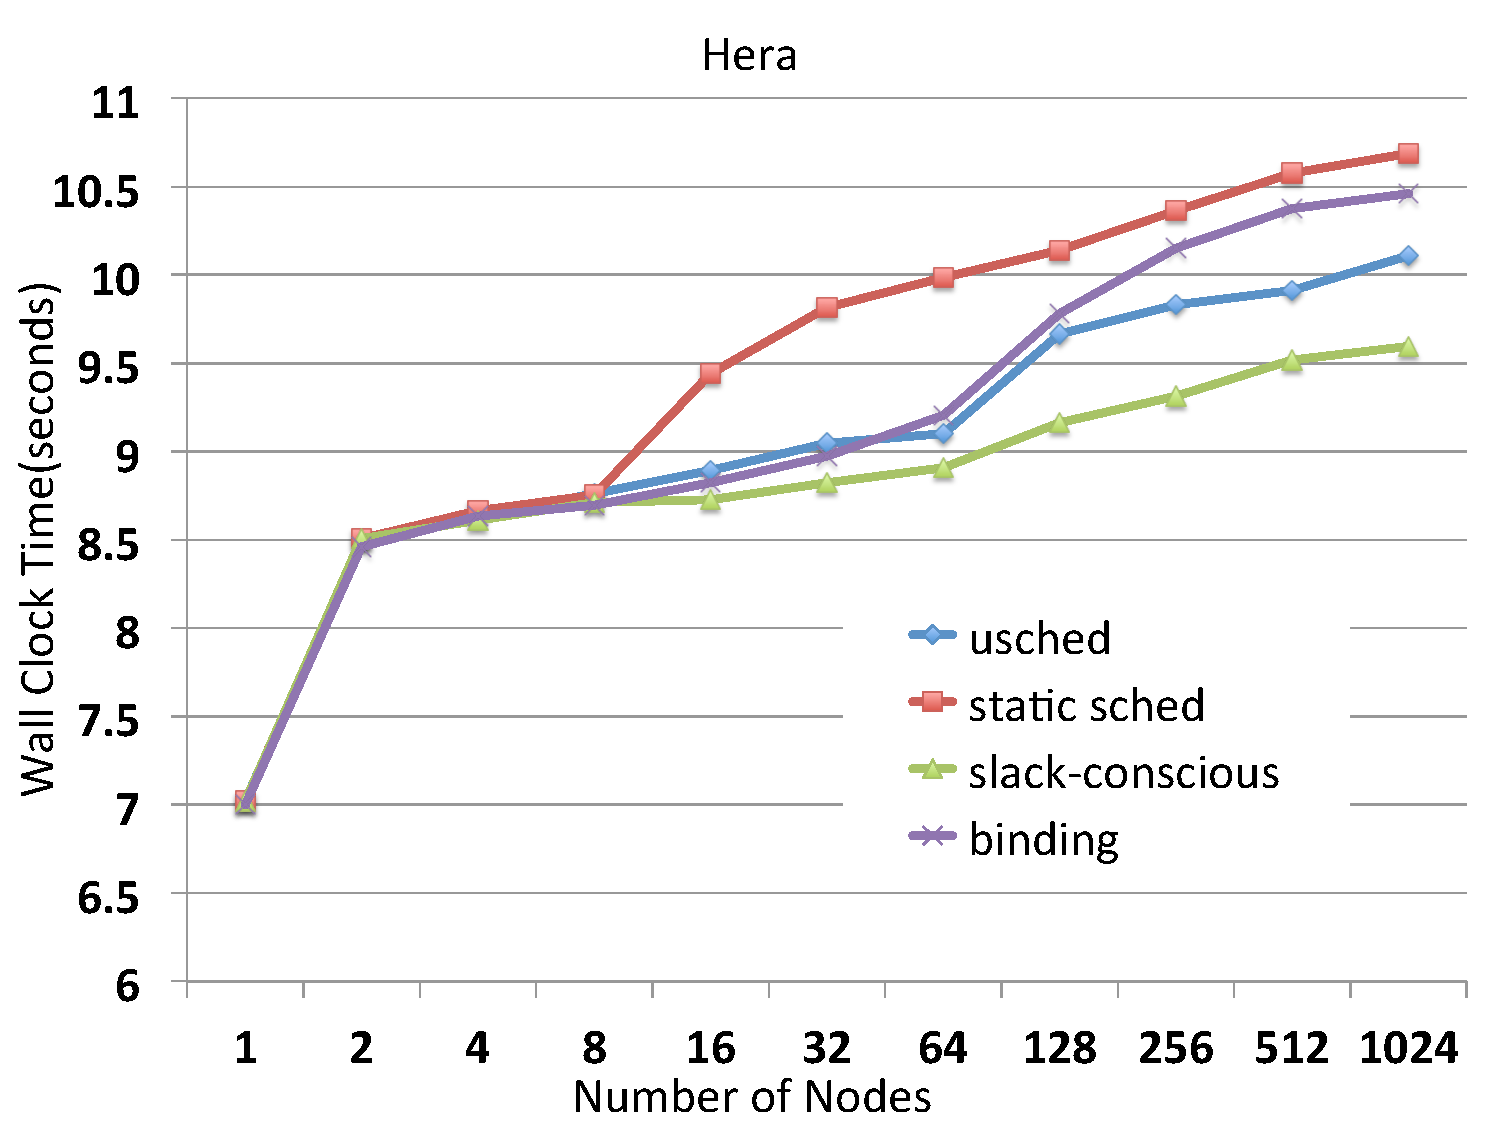
\includegraphics[width=.65\columnwidth]{images/AMG-scaling-hera} 
      \caption{ \small On a machine with 16 cores and medium noise, slack-conscious lightweight scheduling allows for roughly 17\% perf gains over baseline.} 
    \end{figure} 
  \end{block}

  %-- Block 3-3 
  \begin{block}{\small Conclusion}
    \begin{itemize}
    \item \small Noise amplification is serious at scale, and lightweight scheduling is one way to mitigate this noise amplification. 
    \item \small By using static fraction that is different on each node, we can further avoid amplification due to variation of work-stealing.
    \item \small Performance gains are highest as we have more cores per node, even noise is low. 
    \end{itemize}   
  \end{block}     
\end{column}%3  

\end{columns}
 
\end{frame} 
  
\end{document}
